\section{Interface}
\label{chapter 4}

Beside the clock (\textit{clk\_i}) and the reset (\textit{rstn\_i}) signals, we can differentiate two type of signals, the ones going to the datapath (fetch stage) and the ones going to the instruction cache. In figure \ref{fig:diagram} we can see the connections of the icache interface.

\begin{figure}[h]
	\centering
	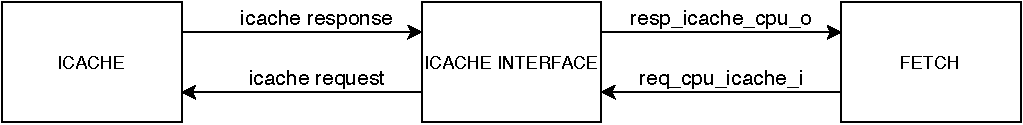
\includegraphics[width=\textwidth]{Figure/diagram}
	\caption{Icache interface block diagram}
	\label{fig:diagram}
\end{figure}


To communicate with the datapath we use the following:

\begin{table}[H]
\centering
\begin{tabular}{llll}
\textbf{Signal name} & \textbf{Width} & \textbf{Type} & \textbf{Description} \\
\hline
req\_cpu\_icache\_i & struct & in & Signals from the CPU \\
resp\_icache\_cpu\_o & struct & out & Response to the CPU \\
\end{tabular}
\end{table}


The signals of the \textit{req\_cpu\_icache\_i} structure are the following:

\begin{table}[H]
	\centering
	\begin{tabular}{llll}
		\textbf{Signal name} & \textbf{Width} & \textbf{Type} & \textbf{Description} \\
		\hline
		valid & 1 & in & Request valid \\
		vaddr & 1 & in & Virtual Addr requested \\
		invalidate\_icache & 1 & in & Petition to invalidate cache content \\
		invalidate\_buffer & 1 & in & Petition to invalidate cache-line buffer \\
	\end{tabular}
\end{table}

The signals of the \textit{resp\_icache\_cpu\_o} structure are the following:
\begin{table}[H]
	\centering
	\begin{tabular}{llll}
		\textbf{Signal name} & \textbf{Width} & \textbf{Type} & \textbf{Description} \\
		\hline
		valid & 1 & out & Response valid \\
		data & 1 & out & Word of 32 bits from Icache \\
		instr\_access\_fault & 1 & out & Upper 24 bits of PC are used. We have 40 bits of PC \\
		instr\_page\_fault & 1 & out & Page Fault from TLB \\
	\end{tabular}
\end{table}

Finally, the icache interface has an obvious connection to the ICache and the signals are the following:

Input Signals (Response from the Icache):


\begin{table}[H]
	\centering
	\begin{tabular}{llll}
		\textbf{Signal name} & \textbf{Width} & \textbf{Type} & \textbf{Description} \\
		\hline
		icache\_resp\_datablock\_i & icache\_line\_t & input & full cacheline requested \\
		icache\_resp\_vaddr\_i & addr\_t & input & addr requested \\    
		icache\_resp\_valid\_i & logic & input & valid response \\
		icache\_req\_ready\_i & logic & input & accepts requests \\
		iptw\_resp\_valid\_i & logic & input & ptw responde valid \\
		ptw\_invalidate\_i & logic & input & ptw invalidation \\
		tlb\_resp\_miss\_i & logic & input & TLB miss \\
		tlb\_resp\_xcp\_if\_i & logic & input & xcpt from ICache \\
		
	\end{tabular}
\end{table}

Output Signals (Request to the Icache):

\begin{table}[H]
	\centering
	\begin{tabular}{llll}
		\textbf{Signal name} & \textbf{Width} & \textbf{Type} & \textbf{Description} \\
		\hline
		icache\_invalidate\_o & logic & output & Invalidate the Icache \\
		icache\_req\_bits\_idx\_o & icache\_idx\_t & output & request addr, index bits \\
		icache\_req\_kill\_o & logic & output & kill current request \\
		icache\_req\_valid\_o & reg & output & request valid \\
		icache\_resp\_ready\_o & reg & output & ready to accept requests \\
		icache\_req\_bits\_vpn\_o & icache\_vpn\_t & output & request addr, vpn bits \\
		tlb\_req\_bits\_vpn\_o & icache\_vpn\_t & output & request bits to TLB \\
		tlb\_req\_valid\_o & logic & output & valid request to TLB \\
		
	\end{tabular}
\end{table}



